% !TeX root = ../main.tex
% Add the above to each chapter to make compiling the PDF easier in some editors.

\chapter{2D Pose Estimation}\label{chapter:2dpose}

2D pose estimation is the first step for this Thesis. Here we explain the rationale behind the 2D and 3D pose separation and the method we used for 2D pose estimation. Lastly, we show the 2D pose results in the gait dataset. 

\section{Decoupling between 2D and 3D pose}

Consider the probabilistic formulation over the variables: the image I, the 3D pose $ \theta \in R^{N\times3} $, the 2D pose $X \in R^{N\times2}$ and camera parameters $ C \in R^{6} $ where N denotes the number of joints and the camera has 3 rotational and 3 translational parameters. Since the 2D pose is produced though the camera model where the 3D pose is projected into a 2D image plane, we can argue that the 3D pose of a human is conditionally independent from the image given the 2D pose ( $p(\theta,C|X,I) = p(\theta,C|X)$ ). This means that the 3D pose estimation can be done solely on basis of 2D joint positions. Although this assumption is not completely accurate it is a good approximation. Monocular cues like depth cues that can be obtained from the image are disregarded with this assumption. We can also argue that the image is produced with a random process which depend on the 2D pose. For the graphical model please see \autoref{fig:graphical-model}.

\begin{figure}[htpb]
    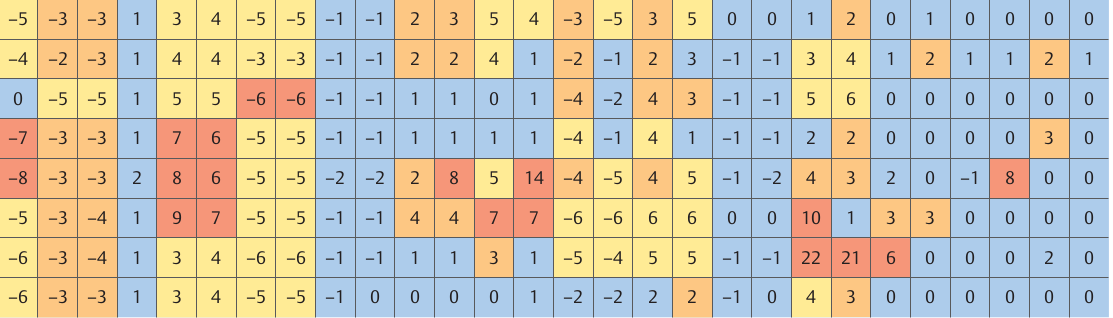
\includegraphics[width=\linewidth]{zmatrix.png}
    \caption{Visualization of the graphical model}
    \label{fig:graphical-model}
\end{figure}

Using Bayes' Rule the joint probability can be written conditioned on the image as follows.

\begin{equation}
    p(\theta,C,X,I) = p(\theta,C,X|I) \cdot p(I)
\end{equation}

The model enables us to expand the joint probabilities as follows

\begin{equation}
    p(\theta,C|X) \cdot p(X|I)= p(\theta,C,X|I)
\end{equation}

Where the task of 3D pose estimation given an image $p(\theta,C,X|I)$ can be thought as a combination of the 2D pose given the image $p(X|I)$ which can be modeled using a Convolutional Neural Network and the 3D pose given the 2D pose $p(\theta,C|X)$ which can be modeled using a Feed-Forward Neural Network. The 2D joint positions act as constraints for the 3D pose which on their own may not be enough to specify a unique pose. However there are other constraints on the human body which limit the ambiguity in the pose and make this assumption practical. 

The main reason behind this process is the lack of computational resources and large and visually variable 3D pose datasets. Since it would be simple to design a model that given an image predicts 3D pose of a human using a Convolutional Neural Network. The model would in principle be able to capture the structure of the human body and give accurate pose predictions in a variety of environments, viewpoints and distances. The combinatorial effect of having many viewpoints, distances and environments would require the dataset to be very large. Limiting the 3D pose estimation to 2D joint locations is a practical and reasonable bottleneck that enables the pose estimation mechanism to work with a small fraction of the required data and processing power. Having the 3D pose estimation model take just 2D points as input opens up the possibility to do augmentation on the viewpoint and distances much easier. 

Training of the a Deep Neural Network becomes more difficult as the depth of the network increases. The training time, inference time and the complexity of the training all increase and make the exploration of different architectures tedious. 
Consider the Human3.6M dataset. Training the model for one set of hyper-parameters would require to process hundreds of millions of images. Which results in a scenario where for one hyper-parameter the training would take more than one day on commodity hardware. In contrast, using the 2D predictions of a off-the-shelf model would require to process the whole dataset only once. Afterwards, one could use the 2D pose estimations as input for developing the 3D pose algorithm which require at least three orders of magnitude less data to process.

One major limitation in the gait dataset is that it has more than 70 million frames of video data. And around 900 frames need to be used to calculate the gait statistics of a single task. This limits our ability to do qualitative evaluations on the entire dataset. Even doing a single pass over data dataset for inference using the video frames is a task that need to be scheduled since it would take on the order of one month on a single GPU. 

This approach has several benefits
\begin{itemize}
    \item It simplifies the pose estimation procedure without sacrificing a lot of the accuracy as it was demonstrated by \parencite{martinez2017simple}, \parencite{sun2017compositional}, \parencite{hossain2017exploiting}
    \item The existing 3D pose datasets do not have the size and visual variability to train a Deep Neural Network that can perform well in in-the-wild scenarios.
    \item This formulation can predict the camera parameters and human pose separately which helps us to train in viewpoint and distance invariant scenarios.
\end{itemize}

\section{Open Pose and results on the Gait dataset}

We decided to use the Open Pose 2D pose detector by Cao et. al. \parencite{cao2016realtime} in the gait dataset. The algorithm is to our knowledge the state-of-the-art in multi-person 2D pose detection. It performs well in in-the-wild scenarios and has algorithmic innovations like Part Affinity Maps that put it in front of other competing methods. It can also run in real-time on commodity hardware. You can see \autoref{tab:mpii-multi-person} for accuracy of comparable methods on the MPII multi person dataset.

\begin{table}[htpb]
    \centering
    \begin{tabular}{l l l l}
      \toprule
        A & B & C & D \\
      \midrule
        1 & 2 & 1 & 2 \\
        2 & 3 & 2 & 3 \\
      \bottomrule
    \end{tabular}
    \caption[2D Pose Comparison]{MPII multi person dataset comparison.}\label{tab:mpii-multi-person}
  \end{table}

The gait dataset contains more than 77000 videos where each video containing around 900 frames. Doing 2D pose inference on more than 70 million frames took around 27 days of GPU time. For such a large amount of data training on the raw data content seems implausible with the current state of hardware limitations. The average joint detection rates can be seen in \autoref{tab:open-pose-gait-rate}.

\begin{table}[htpb]
    \centering
    \begin{tabular}{l l l l}
        \toprule
            A & B & C & D \\
        \midrule
            1 & 2 & 1 & 2 \\
            2 & 3 & 2 & 3 \\
        \bottomrule
    \end{tabular}
    \caption[Joint detection rate]{Joint detection rate of Open pose \parencite{cao2016realtime} on the gait dataset}\label{tab:open-pose-gait-rate}
\end{table}

For qualitative evaluation of the 2D pose estimates we show accurate estimates together with failure cases in \autoref{fig:gait-failure}. The pose prediction has certain obvious limitations some due to the limited view point of the camera and some related with pose prediction algorithm's performance. 

\begin{figure}[htpb]
    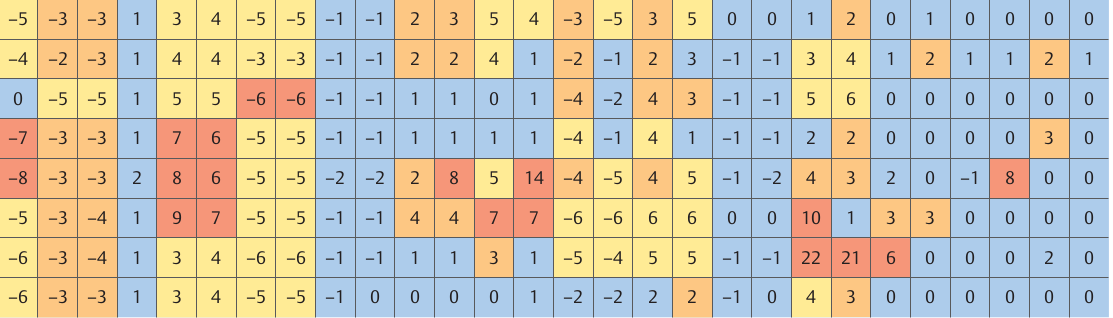
\includegraphics[width=\linewidth]{zmatrix.png}
    \caption{Visualization of the Z-matrix}
    \label{fig:gait-failure}
\end{figure}

\begin{itemize}
    \item The detection is not possible when the subject is not visible in the beginning or in the end of the sequence. See \autoref{fig:gait-failure} and \autoref{fig:gait-failure}
    \item The detection is generally less successful  when the subject turns his or her back to the camera especially the eyes, ears and head detection. \autoref{fig:gait-failure} and\autoref{fig:gait-failure}
    \item There are missing joints during the sequence sometimes in the middle of the sequence. \autoref{fig:gait-failure} and \autoref{fig:gait-failure}
\end{itemize}
